\newpage
\chapter{ÇEKİRDEK SENTEZLENMESİ}\label{ch:cekirdekSentez}
\paragraph{}
ÇÇSN evrende meydana gelen en uç olaylar arasındadır. $ 8$-$9 $ Güneş kütlesinden daha büyük kütleye sahip yıldızlar olağanüstü bir patlama ile ömürlerini sonlandırırlar. Çöken materyalden açığa çıkan kütle çekim bağlanma enerjisi büyük oranda nötrinolar tarafından dışarı aktarılır \cite{1966ApJ...143..626C, 1986ARA&A..24..205W, 1989ARA&A..27..629A}. Enerji emisyonu sırasında dışarı aktarılan enerji yıldız içerisindeki elementleri uzay boşluğuna fırlatır. Bu elementler, yalnızca yıldızın ömrü boyunca hidrostatik yanmadan çıkan ürünlerini değil, aynı zamanda patlama sırasında sentezlenmiş nükleer çekirdeklerdir. Ayrıca, patlama enerjisinin $ \% 99 $'unu taşıyan nötrinolar bazı anahtar elementlerin üretilmesinde de önemli rol oynar. Açığa çıkan nötrinolar ÇÇSN başlamadan önce yıldızın çekirdeğinde termal dengeye gelmiştir. Bundan dolayı nötrinoların sıcaklığından bahsedilebilir. Nötrino sıcaklıkları \ref{tbl:AvaregedProducitionFactors} numaralı şekilde de görüldüğü üzere çeşitlilik gösterebilir. Bu sıcaklıklık farkları da nötrino etkileşimleri ile oluşmuş elementlerin üretiminde önemli rol oynar. Bu tipte etkileşimlere \emph{nu-işlemi} (nu-process) adı verilir.
\begin{table}[hbt!]
    \centering
    \begin{tabular}{|l|l|l|}
    \hline
    Çekirdek    & Düşük Enerji & Yüksek Enerji \\ \hline
    $^{7}$Li    & $ 0.04 $     & $ 0.58 $ \\ \hline
    $^{11}$B    & $ 0.31 $     & $ 1.57 $ \\ \hline
    $^{15}$N    & $ 0.09 $     & $ 0.16 $\\ \hline
    $^{19}$F    & $0.18$       & $ 0.29 $\\ \hline
    $^{138}$La  & $0.46$       & $0.77  $ \\ \hline
    $^{180}$Ta  & $0.49$       & $0.84$ \\ \hline
    \end{tabular} 
    \caption[Solar Bolluğa Göre Ortalama Üretim Faktörleri.]{Solar bolluğa göre ortalama üretim faktörleri \cite{Sieverding:2018rdt}. $ ^{16} $O üretimine göre normalize edilmiştir. Buradaki düşük veya yüksek enerji, sıcaklıklar manasındadır; Düşük enerji için $ T_{\nu_{e}}=2.8 $ MeV, $ T_{\overline{\nu}_{e}}= T_{\nu_{\mu,\tau}}=4.0 $ MeV ve Yüksek enerji için $ T_{\nu_{e}}=4.0 $ MeV, $ T_{\overline{\nu}_{e}}=5.0$ MeV, $ T_{\nu_{\mu,\tau}}=6.0 $ MeV. Burada müon ve tau nötrinoları ve antinötrinoları aynı sıcaklıktadır.}\label{tbl:AvaregedProducitionFactors}
\end{table}

Yıldız evrimi sırasında demir elementine kadar sentezlenen elementlerin, örneğin karbon, oksijen, demir gibi, bolluğunu nükleer tepkimeler yardımı ile açıklayabiliriz \cite{Burbidge:1957vc}. Öte yandan, güneş sisteminde bulunan nadir izotopların sentezlenmesi hala açık bir sorudur. Süpernova sırasında meydana gelen çekirdek sentezi Güneş sistemindeki elementlerin bir kısmının bolluğunu açıklamak için kullanılır. Ancak ÇÇSN'deki nükleer sentezleme hakkındaki bilgimiz patlama modelleri ile sınırlıdır. Çoğunlukla yapay parametreler kullanılarak yapılan patlama modelleri Güneş sistemindeki element bolluğunu tamamen karakterize edemez. Süpernova çekirdek sentezi üzerine çeşitli çalışmalarla yapılmış olsa da, \cite{1954ApJS....1..121H, 1995ApJS..101..181W, 1996ApJ...460..408T}, gözlemlenen süpernova kalıntıları ve evrimleri hala model bağımlıdır veya serbest parametre bağımlıdır. Yıldız evriminde çekirdek sentezi, tek başına demirden daha ağır elementler üretmek için yeterli olmasa da $ ^{7} $Li ve $ ^{11} $B izotopları gibi bazı izotopların üretimini sağlayarak Güneş sistemindeki bilinen elementlerin bolluğuna katkıda bulunur \cite {Sieverding:2018rdt}.

Günümüzde çok boyutlu ÇÇSN simülasyonları, son hesaplama teknolojisindeki gelişmelerle beraber daha ayrıntılı olarak gerçekleştirilebilir \cite{Janka:2017vcp}. Ancak patlama simülasyonlarının çoğu sadece birkaç yüz milisaniye kadar çalışabilir. Geç zaman ÇÇSN soğuma fazında (cooling phase) çekirdek sentezlenme hesapları için yeterli değildir. Biz bu zorlukların üstesinden gelmek için başarılı bir şekilde patlayan PUSHing yöntemi \cite{2015ApJ...806..275P} adlı, tamamen kendisi tutarlı tek boyutlu süpernova modelini kullandık. Bu model ata yıldızı (progenitor) oluşturan elementlerin her bir zaman aralığında dinamik değişimini açıklar ve neredeyse beş saniye boyunca dinamik çekirdek sentezleme hesabının yapılmasına olanak verir.

\section{PUSHing ÇÇSN MODELİ}\label{sec:PUSHing}
\paragraph{}
PUSH (Parametrized Spherically Symmetric Explosion Method) veya PUSHing modeli patlama için yapay olarak tetiklenen tek boyutlu bir ÇÇSN modelidir. Bu modelin ayrıntılı açıklamaları \cite{2015ApJ...806..275P,2019ApJ...870....1E} numaralı kaynaklarında ve PUSH yöntemini kullanarak çekirdek sentezi analizi yapan \cite{Curtis:2018vkh} numaralı kaynakta bulunmaktadır. Bu bölümde kısaca modeli açıklayıp bizim kullandığımız parametreleri vereceğiz. Bu çalışmada tek boyutlu simülasyondan elde edilen başlangıç koşullarını dikkate alınacaktır. İki boyutlu ÇÇSN için \cite{2018JPhCS.940a2054S} numaralı kaynağa başvurabilirsiniz.

PUSH simülasyonu, küresel simetrik başlangıç koşulları ile başlayıp göreli hidrodinamik denklemleri çözen AGILE \cite{Liebendoerfer:2000fw} kodunu kullanmaktadır. Kod nötrino güdümlü (neutrino-driven) mekanizmaya dayanır. Tek boyutlu simülasyonlar herhangi bir türbülans, konveksiyon veya SASI (Standing Accretion Shock Instabilities) oluşturmasa da ÇÇSN'nin temellerini anlamak için uygundur. Üstelik çok boyutlu yöntemlerin bir saniyeden öteye gidemeyecek kadar bilgisayar hesaplama maliyeti vardır. Bilgisayar kaynaklarındaki  hesaplama kısıtlaması tam çekirdek sentezleme sonuçlarını elde etmedeki çok büyük engellerden biridir. Bu nedenle, PUSH gibi parametrize edilmiş yöntemler çekirdek sentezleme hesaplaması için büyük öneme sahiptir. Çok boyutlu simülasyonlarda nötrinoların çeşnilere göre sıcaklıkları ÇÇSN'nın patlayıp patlamamasında kritik rol oynar. Başarılı bir patlama sekme (bouncing) evresinden sonra açığa çıkan şok dalgasının enerjisine bağlıdır. Açığa çıkan nötrinolar şok dalgasını hem ısıtır hem de iter. PUSH metodu şokun kinetik enerjisini besleyen nötrinoların oranını yapay olarak arttırarak şoku besler. Yani nötrinoların sıcaklıklarını arttıran serbest bir parametre kullanır. Bu ısıtmayı betimleyen yerel bir büyüklük tanımlayabiliriz.
\begin{equation}
    Q^{+}_{push}(r,t)=4\mathcal{G}(t) \int_{0}^{\infty}q^{+}_{push}(r,E)dE \text{ .}
\end{equation}
Burada 
\begin{equation} \label{eqn:PUSHartificial}
    q^{+}_{push}(r,E) \equiv \sigma_{0}\frac{1}{m_{b}}\qty(\frac{E}{m_{e}c^{2}})^{2} \frac{1}{4\pi r^{2}} \frac{d L_{\nu_{x}}}{dE} \mathcal{F}(r,E)
\end{equation}
şeklinde tanımlanmıştır. $ \sigma_{0} $, nötrinoların tipik tesir kesiti, $ m_{e,b} $ elektron ve baryon kütlesi, $ (dL_{\nu_{x}}/dE)/(4\pi r^{2}) $ terimi spektral enerji akısı $ \mathcal{G} $ ve $ \mathcal{F} $ terimleri ise PUSH simülasyonundan elde edilen uygun evrim fonksiyonlarıdır. Daha ayrıntılı hesap için \cite{2015ApJ...806..275P} numaralı kaynağı bakınız. 

Müon ve tau nötrinolarının ve antinötrinolarının sıcaklıklarını yapay olarak arttırmak kendisiyle tutarlı (self-consistent) süpernova patlaması meydana getirmektedir. Buradaki simülasyonu tetikleyen tüm parametreler, Süpernova \textit{SN1987A} 'dan esinlenmiştir. Sonuç olarak $ 18.8 $ Güneş kütlesine sahip bir ata yıldız kullanarak yaptığımız simülasyonun başlangıç parametreleri numaralı tabloda verilmiştir.
\begin{table}[hbt!]
    \centering
    \begin{tabular}{|l|l|}
    \hline
    \textbf{Parametreler} & \textbf{Değerler} \\ \hline
    Ata Yıldızın Kütlesi & 18.8 M$_{\odot}$ \\ \hline
    Kütle Kesimi (Mass Cut) & 1.5466 \\ \hline
    İzleyici (Tracer) Çıktı Sayısı & 3146 \\ \hline
    Kütle Hassasiyeti & 10$ ^{-3} $M$_{\odot}$\\ \hline
    Patlama Zamanı & $ \sim $ 4 s \\ \hline
    Patlama Enerjisi & 1.2$\times  $10$ ^{51} $ erg \\ \hline
    \end{tabular} 
    \caption[PUSH Modelinin Parametreleri.]{PUSH Modelinin Parametreleri.} 
    \label{table:ProgenitorParameters}
\end{table}

Bizim kullandığımız ata yıldız modelinde dış katmanların verisi bulunmamaktadır. \ref{fig:progenitorAbund_Temp} numaralı şekilden de görüleceği üzere, yıldızın en büyük katmanı olan Helyum (HE) katmanı çok küçük gözükmektedir. Bu şekilde almamızın sebebi simülasyonun $ t=4 $ s'de sonlaması ve şok dalgasının yaklaşık O/C katmanına gelmesidir. Yani bu katmandan sonrasında çekirdek sentezlenmesinin başlamamasıdır. \ref{fig:progenitorAbund_Temp} numaralı şekilde, tepe sıcaklığının $ t=5 $ s'deki dağılımı ve ata yıldızın (simülasyon başlamadan önceki hali) katmanları içerisindeki bazı elementlerin kütle oranlarını gösterilmektedir. Tepe sıcaklık grafiğinde, O/C katmanındaki ani değişimin sebebi şok dalgasıdır. Yani şok dalgası $ t=5 $ s süre geçtiğinde yaklaşık $3.8$ - $4.2$ Lagranjiyen kütle koordinatlarında bulunmaktadır. Grafikte arka planda bulunan renkler süpernova içerisindeki katmanları göstermektedir; Mavi Si katmanını, sarı O/Ne katmanını, mor O/C katmanını ve yeşil ise He katmanını gösterir. 

\begin{figure}[hbt!]
	\centering
	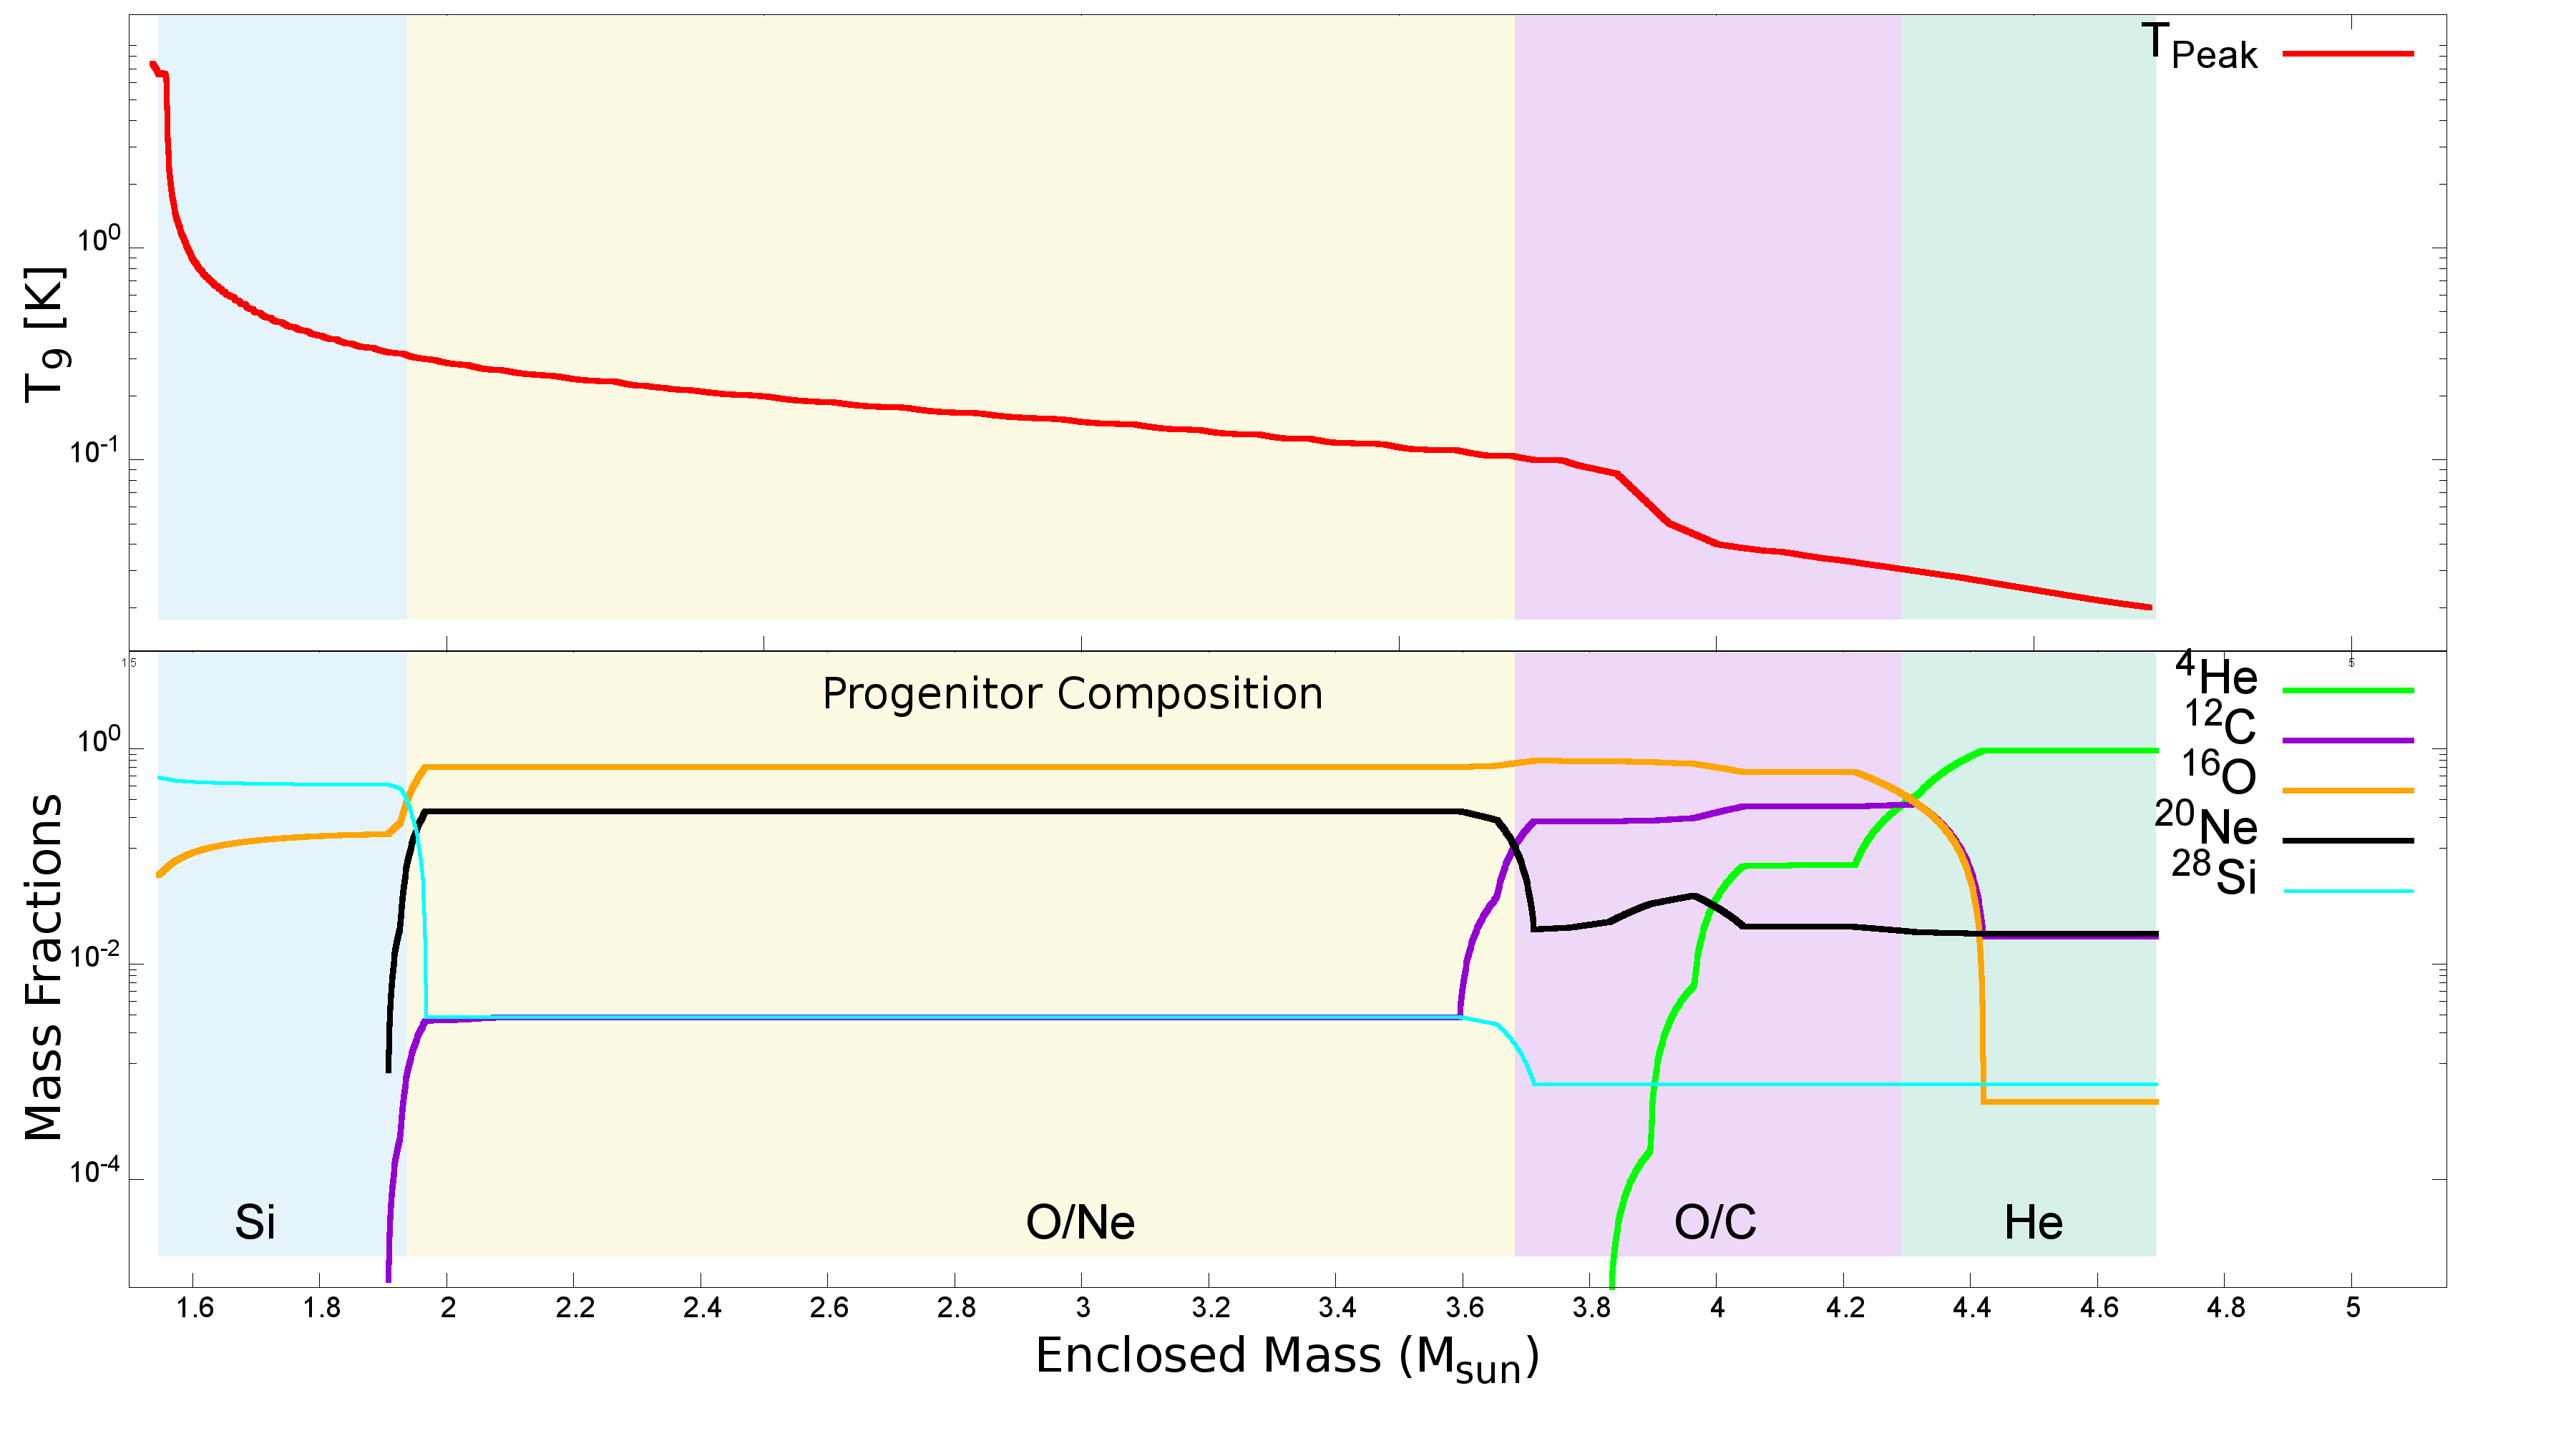
\includegraphics[width=\textwidth]{figures/progenitorAbund_Temp.png}
	\caption[Ata Yıldızın Bolluğu Ve Tepe (Peak) Sıcaklığı.]{Ata yıldızın bolluğu ve tepe (peak) sıcaklığı. Çekirdek sentez ağ simülasyonu, $ 6.5 $ GK sıcaklığında nükleer istatistiksel dengededir (nuclear statistical equilibrium.) Bu da yaklaşık Si katmanının ortasına denk gelir.}
	\label{fig:progenitorAbund_Temp}
\end{figure}

Tepe sıcaklığının nükleer istatistiksel dengeyi nasıl etkilediğini ve çekirdek sentezlenme hakkındaki detayları göreceğiz. Bunun için termonükleer reaksiyon ağı (thermonuclear reaction network) oluşturmamız gerekecektir.

\section{TERMONÜKLEER REAKSİYON AĞI}\label{sec:termoNukleerReakAg}
\paragraph{}
Termodinamik değişkenleri belirlemek için sadece çekirdek bolluğuna ek olarak büyük ölçekli termonükleer reaksiyon ağına ihtiyaç duyulur. Bu bölümde, çiftlenmiş adi diferansiyel denklemler kümesi olan termonükleer reaksiyon ağı evrimlerini inceleyeceğiz.

Başlangıç noktası olarak en genel reaksiyonu yazalım.
\begin{equation}
    \dots a+B \rightarrow C+d+ \dots \text{ .}
\end{equation}

Reaksiyon çeşitlerini, transfer reaksiyonları ($ ^{15}N(p,\alpha)^{12}C $), yakalama (capture) reaksiyonları ($ ^{3}He(\alpha,\gamma)^{7}Be $), zayıf reaksiyonlar ($ p(p,e^{+}\nu_{e})d $) veya bozunumlar ($ ^{56}Ni\rightarrow^{56}Co+e^{+}+\nu_{e} $) olarak kategorize edebiliriz. Bunlara ek olarak üçlü $ \alpha $-işlemi gibi, üç çekirdekten oluşan reaksiyonlar da önemlidir. Reaksiyon sonucunda her bir tepkiyen (reactant) sayı yoğunluğu, $ n_{i} $, zamanla ve reaksiyon hızı, $ r $, ile değişecektir.
\begin{equation}\label{eqn:networkDif1}
    \frac{d n_{i}}{d t}=\sum_{j} \mathcal{N}^{i}_{j}r_{j}+\sum_{j,k} \mathcal{N}^{i}_{j,k}r_{j,k}+\sum_{j,k,l} \mathcal{N}^{i}_{j,k,l}r_{j,k,l} \text{ .}
\end{equation}

Enerji-momentumun ve toplam elektrik yükün ağ hesaplaması sırasında korunması gerekmektedir. Burada  $ \mathcal{N} $ pozitif olursa oluşum (creation) negatif olursa yıkım (destruction) tepkimesi olur. $ \mathcal{N} $ ifadesinin tanımı 
\begin{equation}
    \mathcal{N}^{i}_{i}=N_{i},\quad \mathcal{N}^{i}_{j,k}=\pm \frac{N_{i}}{\abs{N_{j} }!\abs{N_{k} }!}\quad \dots
\end{equation}
şeklinde olur. Bu ifadede pay kısmı ayırt edilemez (indistinguishable) parçacık sayımından gelmektedir.

Sayı yoğunluğunu her bir çekirdeğin bolluğuna dönüştürmek için yeni değişkenler tanımlamamız gerekir. Her şeyden önce, her bir çekirdeğin nükleer bolluğu veya molar kesri $ \mathbf{Y}_{i}=\frac{n_{i}}{\rho N_{a}} $ şeklinde tanımlanır. Burada $ \rho $ yoğunluk, $ N_{a} $ ise Avagadro sayısıdır. Her reaksiyon tipi için reaksiyon hızı $ r $ değişecektir. Örneğin yavru çekirdeklerin (daughter nuclei) bozunmasında veya kütlesiz parçacıklar ile reaksiyona girmesinde reaksiyon hızı $ r_{i}=\lambda Y_{i} $ şeklinde yazılır ki $ \lambda $ bahsedilen reaksiyonun bozunma hızıdır. Eğer \eqref{eqn:networkDif1} numaralı denklemi tekrar yazarsak,
\begin{equation}\label{eqn:networkDif2}
    \frac{d Y_{i}}{dt}=\sum_{j}  \mathcal{N}^{i}_{j} \lambda_{j}Y_{j}+ \sum_{j,k} \mathcal{N}^{i}_{j,k} \qty(\frac{\rho}{m_{a}}) \expval{j,k}Y_{j}Y_{k}+ \sum_{j,k,l} \mathcal{N}^{i}_{j,k,l}\qty(\frac{\rho}{m_{a}})^{2} \expval{j,k,l}Y_{j}Y_{k}Y_{l} \text{ ,} 
\end{equation}
ifadesini elde ederiz. Burada $ \expval{i,j} $ yıldızsal (stellar) reaksiyon hızıdır. Bozunma hızı $ \lambda $ ise bozunan parçacığın bozunma hızı ile orantılıdır. Bu değerler hem sayısal simülasyonlarla hem de deneylerle elde edilir. Üç cisim etkileşimleri (three-body interactions) nadiren meydana gelmesine rağmen dikkate alındığında sonuçlarda dramatik etkiye sebep olacaktır. Yukarıda bahsedilen kütle kesri ise $ X_{i}=A_{i}Yi=\frac{\rho_{i}}{\rho} $ şeklinde tanımlanmıştır. Denklemlerdeki baryon korunumunu sağlamak için $ \sum_{i}Y_{i}A_{i}=1 $ ifadesi her an sağlanmalıdır.

Ağı betimleyen \eqref{eqn:networkDif2} numaralı denklem takımını çözebilmek için başlangıç yoğunluğunu ortamın sıcaklığı bilinmelidir. Ayrıca, başlangıçtaki madde bileşimi ve elektron kesri $ Y_{e} $, yani ata yıldızın içeriği hakkında da bilgi sahibi olunması gerekecektir. Eğer sıcaklık ve yoğunluk yeteri kadar yüksek ise nükleer reaksiyonlar iki taraflı olacaktır. Yani yıkım ve oluşum reaksiyon hızları eşit olacaktır ($ \beta $ bozunumu hariç.) Bu durumda ortamdaki madde \emph{nükleer istatistiksel dengeye} (NİD) ulaşmış olacaktır. NİD'de çekirdek sentezlenmesi olmaz. Çekirdek sentezleme hesaplama zamanını azaltmak için nükleer ağ kodu NİD'den çıktığı noktadan başlar. Bu çalışmada NİD sıcaklığı $ 6.5 $ GK civarıdır ve ağ simülasyon kodu $ 6.5 $ GK'den düşük noktalarda çalışacaktır. Böylece gereksiz ve çok katı salınan (stiff) diferansiyel denklem sistemi çözmemize gerek kalmayacaktır.

Nötrino-çekirdek etkileşimleri düşük tesir kesitlerinden dolayı ihmal edilmektedir. Diğer taraftan ÇÇSN'nın merkeze yakın noktalarında nötrino-çekirdek etkileşimlerinin etkileri görülebilir. Bu etkileşimler yüklü ve yüksüz etkileşimler olacaktır. \ref{sec:maddeIleEtkilesim} bölümünde kütleli nötrinolar için etkileşim potansiyelleri ve Hamiltonyenler'i verilmiştir. Tezin çekirdek sentezi bölümünde ise nötrinolar kütlesiz parçacıklar olarak alınacaktır. Nötrino salınımlar dikkate alınarak yapılan çalışmalar için \cite{Wu:2014kaa,Kusakabe:2019znq} numaralı kaynaklarına bakınız. Bu durumda nötrinolar da fotonlar gibi davranacak ancak Fermi-Dirac istatistiğine uyacaktır. Ayrıca elektromanyetik etkileşime de girmeyecekler. Nötrinoların reaksiyon hızı 
\begin{equation}
    \lambda_{\nu}=N\expval{\sigma \phi(E_{\nu},T_{\nu})}
    \end{equation}
şeklinde verilir.

\section{NÖTRİNO İŞLEMİ}\label{sec:NotrinoIslem}
\paragraph{}
Süpernova nötrinoları, proto-nötron yıldızının içinde termal ve kimyasal dengededir. Patlama sırasında nötrinosferden çıkan nötrinolar, sıcak ve yoğun yıldız ortamından geçerler. Nötrinoların tipik tesit kesiti çok küçük olsa bile, nötrino-çekirdek etkileşimi aşırı koşullarda önemli hale gelir. Aslında, yüksüz akım etkileşimi ile çekirdeği uyarabilecek veya yüklü akım etkileşimi ile proton/nötron sayısını değiştirebilecek kadar enerjiye sahiptirler. Bu etkileşimler, çekirdek sentezlenme sürecini etkiler \cite{Woosley:1989bd}. Nötrinoların yoğun madde içerisinde çekirdek sentezleme olayına kısaca \textit{nötrino işlemi} veya \emph{$ \nu $-işlemi} adı verilir. Bu bölümde nötrino işlemini kısaca tanıtacağız ve çekirdek sentezleme hesaplamalarımızın sonucunu özetleyeceğiz.

Birçok $ \nu $-işlem çekirdek sentezleme çalışmasında, nötrinolardan kaynaklanan çekirdek üretimini belirlemenin iki yolu vardır. Birincisi, nötrinolar yeni çekirdekleri doğrudan sentezleyebilir, örneğin, $ ^{12} $C($ \nu\text{ ,}\nu p $)$ ^{11} $B tepkimesi sayesinde. Karbon 12 atomları, nötrinolar tarafından yüksüz akım yoluyla uyarılır ve uyarılmış karbon, bir proton ile boron 11'e bozunur. Bu etkileşim esas olarak $ ^{11} $B elde etmekten sorumludur. İkinci olarak, nötrinolar, $ ^{7} $Li ve $ ^{26} $Al gibi bazı çekirdek bolluklarını önemli ölçüde değiştirebilen parçalanma reaksiyonunun hızını artırabilir \cite{Sieverding:2018rdt}.

$ ^{7} $Li ve $ ^{11} $B hafif elementlerinin kırılgan yapıları nedeniyle yıldız ortamında üretilmesi zordur. Bu çekirdekler, yüklü akım etkileşimleriyle kolayca yok edilir. Öte yandan, $ ^{7} $Li ve $ ^{11} $B çekirdeklerinin Güneş içerisindeki bollukları açıklamak için bir mekanizmaya ihtiyaç duyulmaktadır \cite{2003ApJ...591.1220L}. ÇÇSN içerisindeki nötrino işlemi, hafif çekirdek üretimini açıklamak için en umut verici mekanizmadır. Çekirdek sentezleme ağı hem yüksüz hem de yüklü akım etkileşimlerini içerir. Bahsedilen sentez ağı \ref{fig:li7b11Network} numaralı şekilde gözükmektedir.

\begin{figure}[hbt!]
	\centering
	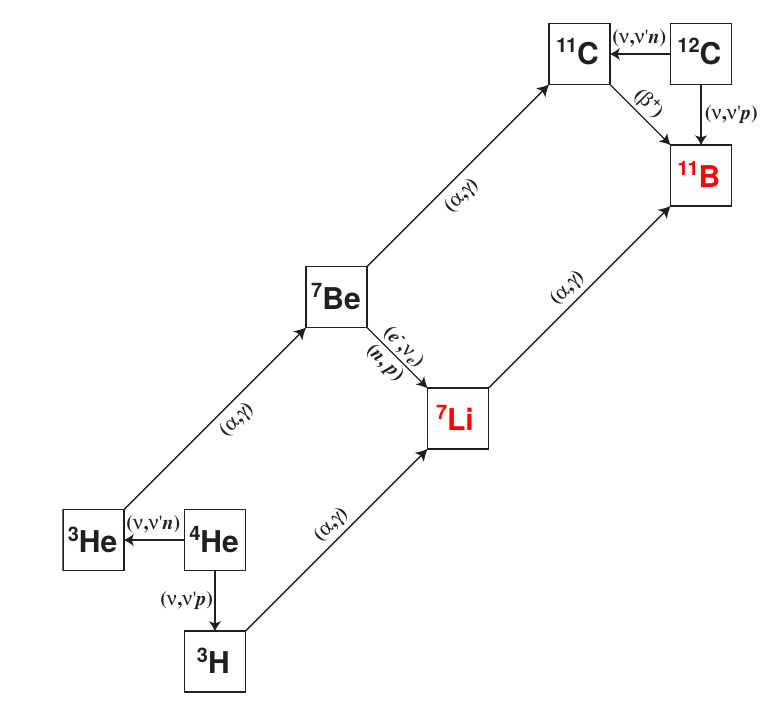
\includegraphics[width=\textwidth]{figures/li7B11_diagram}
	\caption[$ ^{7} $Li ve $ ^{11} $B Çekirdeklerinin Sentezleme Şeması.]{$ ^{7} $Li ve $ ^{11} $B çekirdeklerinin sentezleme şeması. Bu şekil \cite{Suzuki:2006qd} numaralı kaynaktan şekilden esinlenerek çizilmiştir.}
	\label{fig:li7b11Network}
\end{figure}

Nötrino işlemi çekirdek sentezlenmesinde, sadece nötrinoların akısı nihai bollukları etkilemekle kalmaz, aynı zamanda nötrino enerji spektrumu da üretim faktörlerini değiştirir. \cite{Sieverding:2018rdt} numaralı makaleye göre, yüksek enerjili nötrinolar için ortalama $ ^{7} $Li üretim faktörü, düşük enerjilerden on kat daha büyüktür (bkz. \ref{tbl:AvaregedProducitionFactors} numaralı tablo.) Bu dramatik farklılığın nedeni, yüksüz akım etkileşimlerinin büyük ölçüde nötrino enerjilerine bağlı olmasıdır. Bunun yanında $ ^{138} $La gibi çekirdekler, yüksüz akım etkileşiminden iki kat daha fazla oranda yüklü akım etkileşimleri ile üretilir. Bu nedenle, tüm $ \nu $-işlem çekirdekleri ayrı ayrı incelenmelidir.

\section{NÖTRİNO-İŞLEM SİMÜLASYON SONUÇLARI}\label{sec:NotrinoIslemSimSonuc}
\paragraph{}
Yapılan nötrino-işlem simülasyon sonuçlarını irdelemeden önce, PUSHing ÇÇSN model parametrelerinin netleştirilmesi gerekir. Çekirdek sentezi kodu tarafından kullanılan bazı termodinamik değişkenler aşağıda açıklanmıştır. Patlama sırasında nötrinoların sıcaklığı ve parlaklığı, patlamanın hangi fazda olduğuna, yani zamana göre değişir. Proto-nötron yıldızının içi, nükleer yoğunlukta olduğundan nötrinolar termal dengeye ulaşır. ÇÇSN simülasyonunun başlangıcında nötrinosferden yayılan nötrinolar görece soğuktur. Nicelik olarak değerleri \ref{fig:nuTemp} numaralı şekilde gösterilmiştir. Bir süre sonra demir çekirdek çöker ve birkaç milisaniye içinde çöken malzeme, proto-nötron çekirdeğine çarpar ve seker (bouncing.) Sekmenin hemen ardından şok dalgası oluşur. Açığa çıkan nötrinoların sıcaklığı $50$ MeV'e kadar çıkar. Buraya kadar olan olaylara \emph{patlama} (explosion) adı verilir ve patlamanın başlangıcı, sekmenin olduğu andır. Sekme fazının akabinde sıcak nötrinolar, proto-nötron yıldızının yakınındaki malzemeyi ısıtır ve onları uzaya doğru iter. Nötrinolar yardımıyla şok dalgasını ısıtmak ve iç malzemeyi dışarı itmek \emph{nötrino güdümlü mekanizma} (neutrino driven mechanism) olarak adlandırılır. Nötrinoların parlaklığı, evrendeki en uç değerlerden biri olan $10^{58} $ erg/s'ye ulaşır. Her bir nötrino tipinin parlaklıkları şekil \ref{fig:nuLum}'da gösterilmiştir.

\begin{figure}[hbt!]
    \centering
    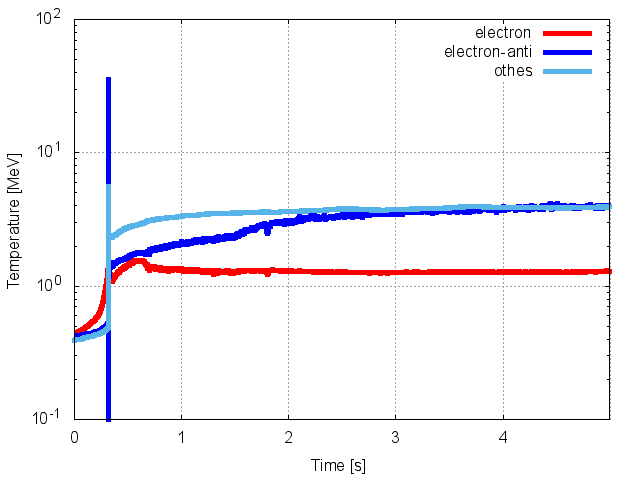
\includegraphics[width=\textwidth]{figures/nuTemperature}
    \caption[ÇÇSN Simülasyonunda Açığa Çıkan Her Nötrino Çeşnisinin Sıcaklığı]{ÇÇSN Simülasyonunda açığa çıkan her nötrino çeşnisinin sıcaklığı. Sıcaklığın $ 10^{-3} $ MeV civarına düştüğü an sekmenin olduğu andır ve bu dramatik değişim sayısal hatadan kaynaklanır. Sekme öncesinde elektron çeşnisinin sıcaklığı yüksek iken patlamadan sonra elektron çeşnisinin sıcaklığı düşük olur. Bu sıcaklık farkının en önemli sebebi nötrinoların küçük tesir kesitinin çeşniye göre küçük farklılıklar oluşturmasıdır. Elektron nötrinosunun tesir kesiti diğerlerine göre büyüktür ve proto-nötron yıldızından ısıl olarak ayrışması daha dış katmanlarda olur. Bu da elektron nötrino sıcaklığının düşük olmasına sebep olur. Daha ayrıntılı bilgi için \cite{Mathews:2014qba} numaralı kaynağın içeriğine ve bu kaynaktaki 3 numaralı şekle bakınız.}
    \label{fig:nuTemp}
\end{figure}
\begin{figure}[hbt!]
    \centering
    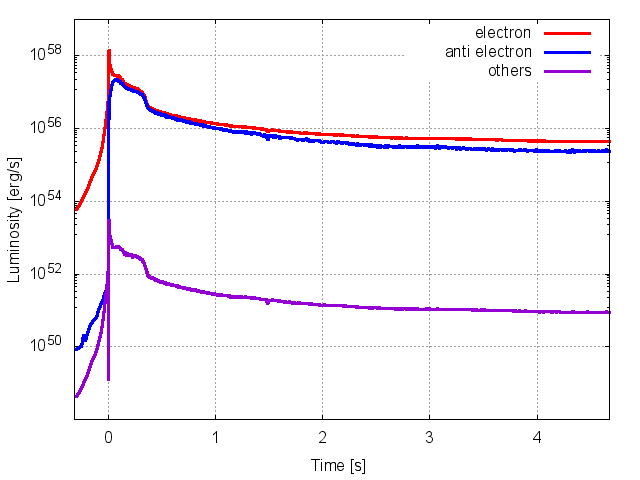
\includegraphics[width=0.7\textwidth]{figures/nuLuminosity}
    \caption[ÇÇSN Simülasyonunda Açığa Çıkan Her Nötrino Çeşnisinin Akısı.]{ÇÇSN simülasyonunda açığa çıkan her nötrino çeşnisinin. Bu şekilde, ÇÇSN'nın başlama zamanı $ 0 $ s'dir ve \eqref{fig:nuTemp} numaralı şekilde gözüken sayısal hata bu grafikte de mevcuttur.}
    \label{fig:nuLum}
\end{figure}

Sonuçlar, ortamın sıcaklığını ve yoğunluğunu, izleyicilerin mesafe değişimini, elektron fraksiyonunu, her bir nötrino çeşnisinin parlaklığını ve her bir SN izleyicisi için geçerli sıcaklıkları (zamana bağlı) içermektedir. Ayrıca $n$, $p$, $ ^{3} $He, $ ^{4} $He, $ ^{12} $C, $ ^{14} $N, $ ^{16}O, $, $^{20} $Ne, $ ^{24} $Mg, $ ^{28} $Si, $ ^{32} $S, $ ^{36} $S, $ ^{36} $Ar, $ ^{ 40} $Ca, $ ^{44} $Ti, $ ^{48} $Cr, $ ^{50} $Ti, $ ^{52} $Fe, $ ^{54} $Fe, $ ^{56} $Fe, $ ^{56} $Ni, $ ^{58} $Fe, $ ^{60} $Fe, $ ^{62} $Fe ve $ ^{62} $Ni çekirdeklerinin bollukları başlangıç koşulu olarak verilir. Bu çekirdekler, ata yıldızın kütlesine bağlı olarak yıldız evriminde üretilmiştir. Ata yıldızın içeriğindeki tüm çekirdekler dahil edilmemektedir, yani daha yüksek kütleli ata yıldız modelleri dikkate alınmadığı için, ağır izotoplar olmak üzere birçok radyoaktif izotopu hariç tutuyoruz. Bu ağır izotoplar, ağır $ \nu $-elementler üretmemizi sağlayacaktır. Temel olarak, çekirdek sentezleme kodu, her izleyicinin içerisinde bulunan her izotop için çiftlenmiş diferansiyel denklemler çözer. Çalıştırılan kodda $1988$ farklı çekirdek türü ve $3146$ izleyiciyi bulunmaktadır. Bu çekirdek türlerin bazılarının bollukları sıfırdır. Bol sıfır bulunan diferansiyel denklem sistemleri çözmek için seyrek matris (sparse matrix) tekniği kullanılır. Bu teknik sayesinde büyük miktarda bilgisayar gücünden tasarruf edilir. Çekirdek sentezleme kodunun çözümleri daha hızlı analiz etmek ve genel sentezleme eğilimine bakmak için, bu çalışmayı $ ^{7} $Li, $ ^{11} $B, $ ^{15} $N ve $ ^{19} $F gibi hafif $ \nu $-işlemi elemanlarını analiz etmekle sınırlandırdık.

SN modelinin özellikleri \ref{table:ProgenitorParameters} numaralı tabloda ve başlangıç kütle kesirleri ise \ref{fig:progenitorAbund_Temp} numaralı şekilde (alt panel) verilmiştir. Ata yıldızın bileşimi ve termodinamik değişkenler patlama için uygundur. Bunun anlamı kullandığımız ÇÇSN modeli başarıyla patlamaktadır. \cite{Sieverding:2018rdt} numaralı kaynak ve \cite{Kusakabe:2019znq} numaralı kaynaktan farklı olarak, $ ^{12} $C çekirdeğinin başlangıç bolluğu, O/Ne bölgesinin sonunda keskin bir şekilde artmaz. Bu da, o bölgedeki $ ^{7} $Li ve $ ^{11} $B üretim oranını değiştirir.
\begin{figure}[hbt!]
    \centering
    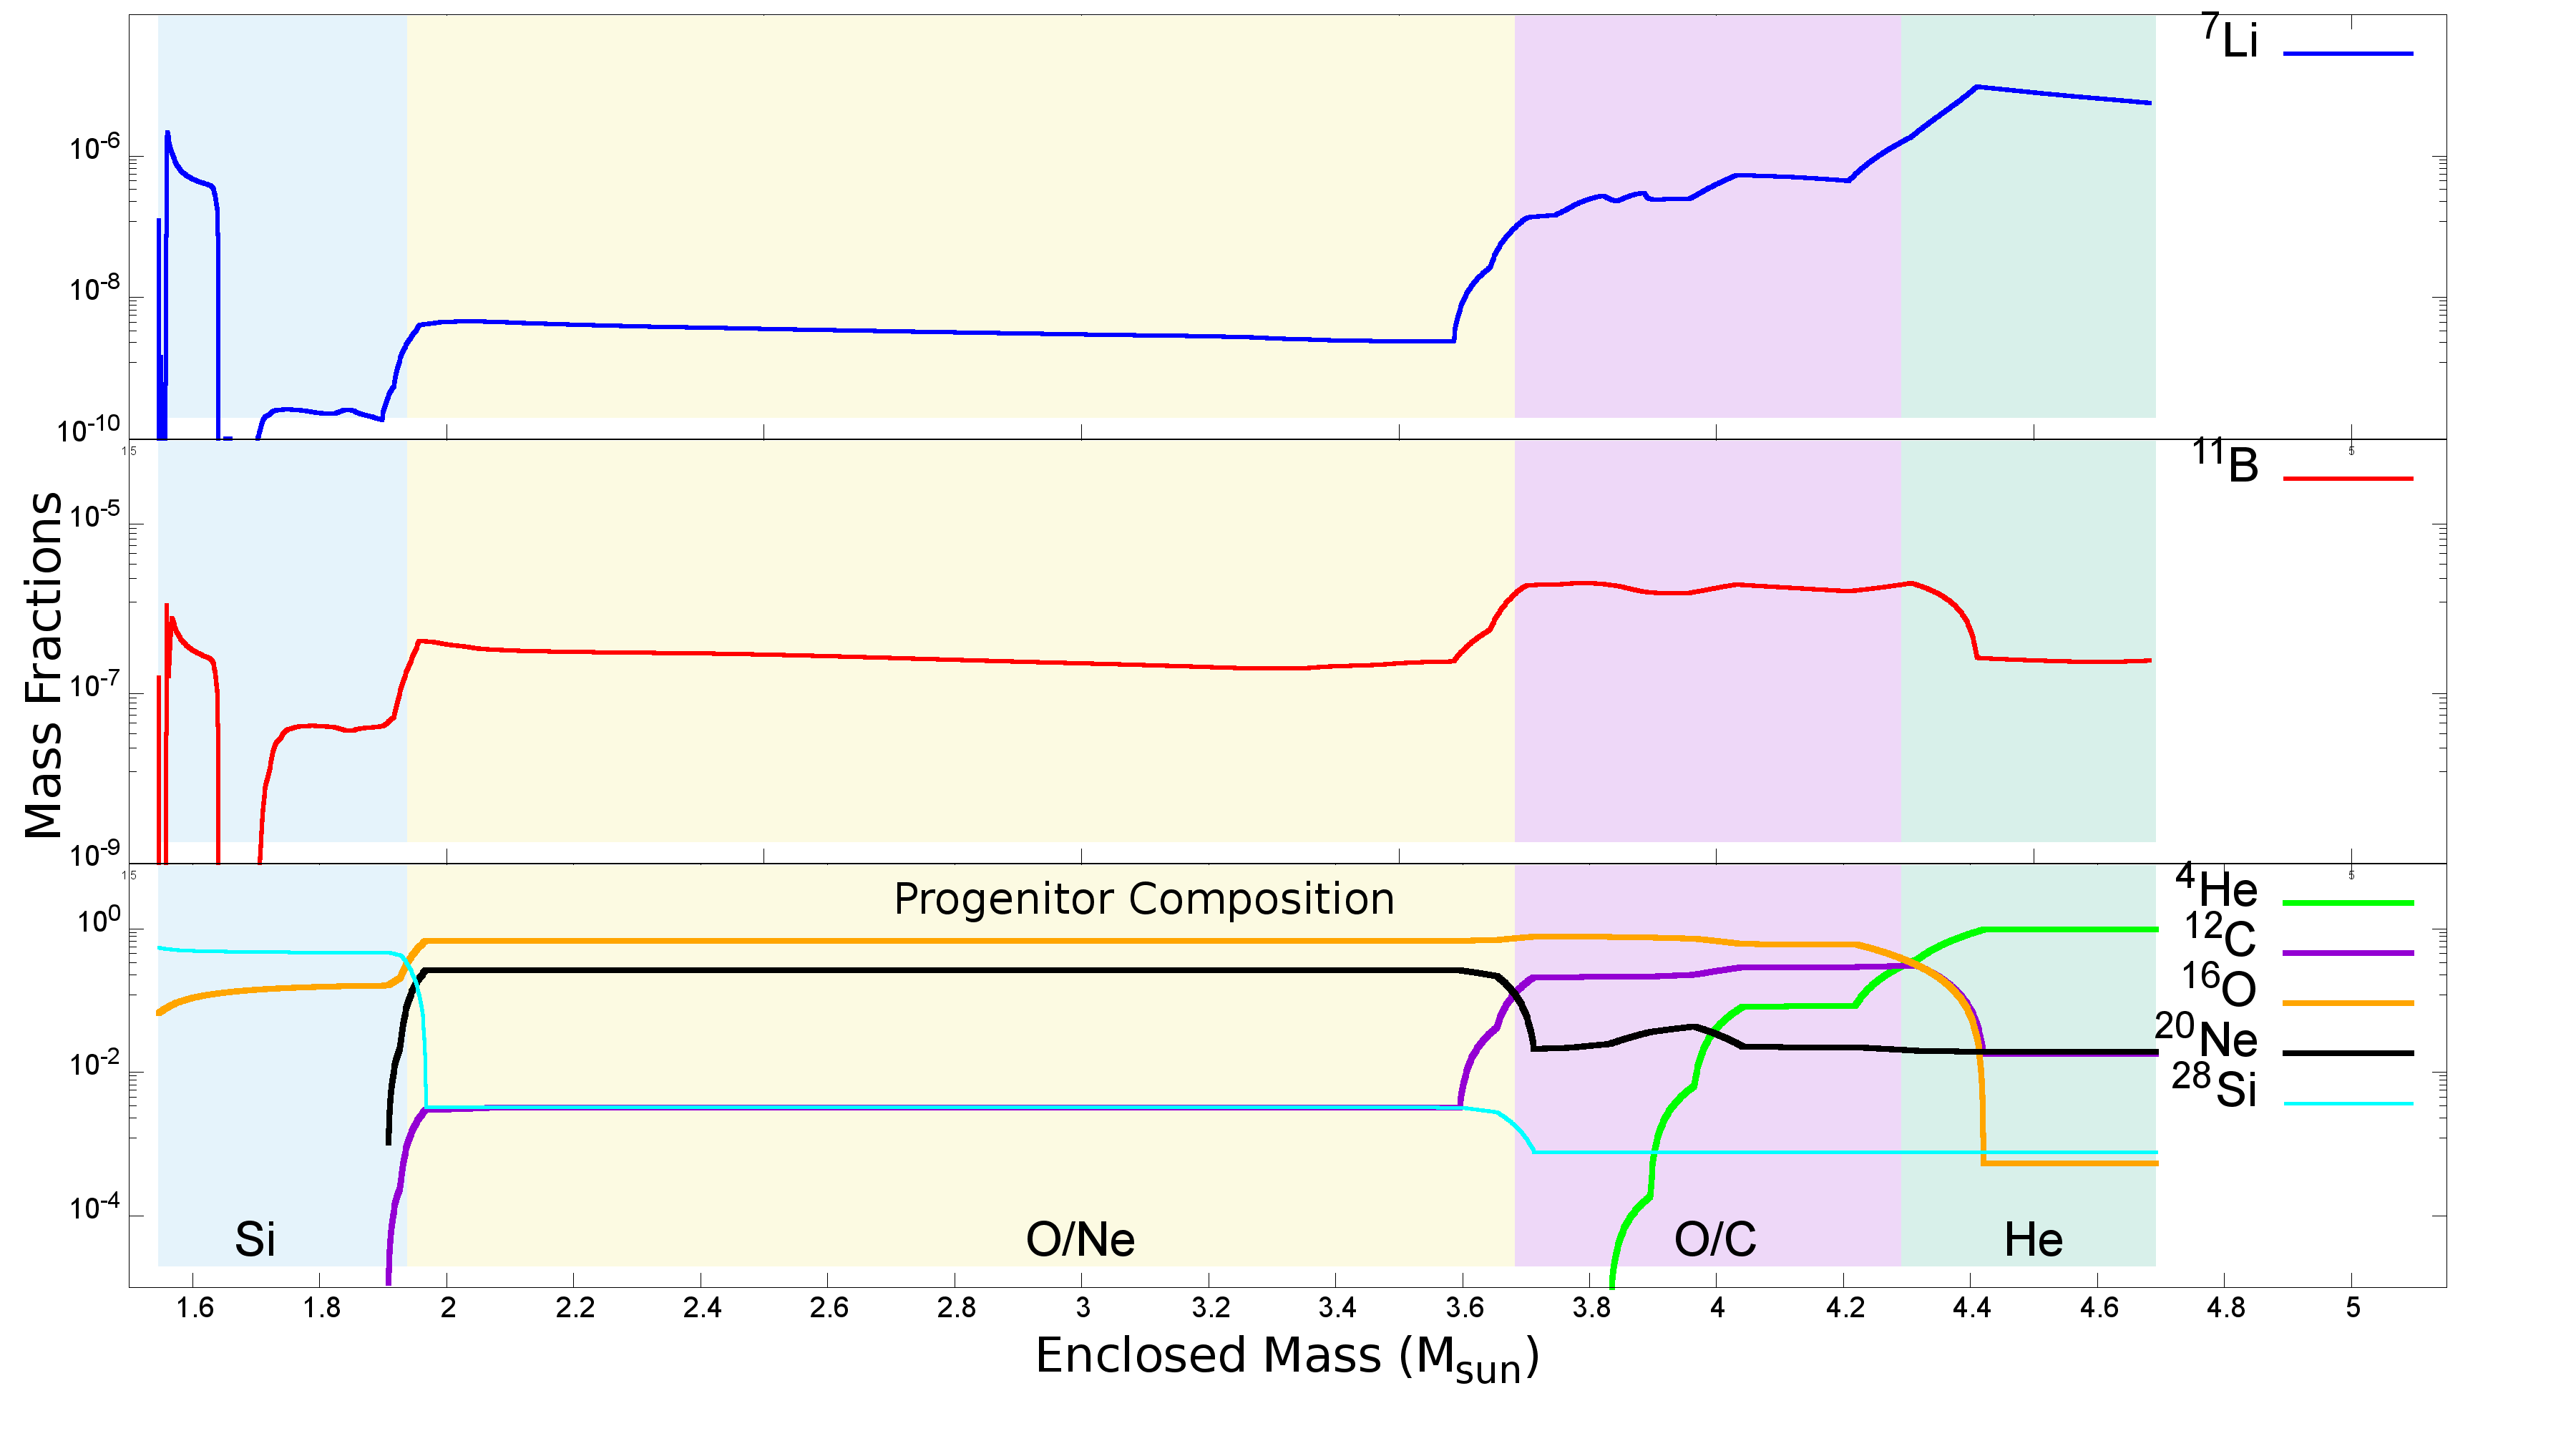
\includegraphics[width=\textwidth]{figures/abundadecay_li7b11}
    \caption[$ ^{7} $Li ve $ ^{11} $B Çekirdeklerinin Kütle Kesirleri.]{$ ^{7} $Li ve $ ^{11} $B çekirdeklerinin kütle kesirleri. Burada $ ^{7} $Li ve $ ^{11} $B üretimleri O/C katmanında arttığı görülmektedir.}\label{fig:abundadecay_li7b11}
\end{figure}

\ref{fig:abundadecay_li7b11} numaralı şekilde, $ ^{7} $Li ve $ ^{11} $B çekirdeklerinin SN katmanlarına göre karakteristik üretimi gösterilmektedir. $ ^{7} $Li bolluğunun yükselişi Si katmanında başlar ancak O/Ne katmanında sabit kalır. Çok iç bölgede (inner most region), $ ^{7} $Li ve $ ^{11} $B çekirdeklerinin ana üretim mekanizmaları, $ ^{7} $Li için $ ^{3} $He($ \alpha $,$\gamma$)$ ^{7} $Be( $ \beta^{+} $)$ ^{7} $Li ve $ ^{11} $B için $ ^{3} $H($ \alpha $,$ \gamma $)$ ^{7} $Li ($ \alpha $,$ \gamma $)$ ^{11} $B tepkimeleridir. Çok iç bölgedeki bileşiminde yeterli $ ^{4} $He çekirdeği yok gibi görünse de, ÇÇSN patlama mekanizması ile bu bölgede yüksek miktarda $ \alpha $ parçacığı asılı kalır. Bu duruma \emph{$ \alpha $-zengin dondurması} ($\alpha$-rich freeze-out) adı verilir. Ayrıca, Si katmanındaki nötrino akısı, dış katmanlardan çok daha büyüktür. Nötrinolar O/C ve He katmanlarına geldiğinde, şekil \ref{fig:li7b11Network}'deki tüm etkileşimler çok hızlı gerçekleştiği için çekirdek bollukları tekrar artacaktır. $ ^{4} $He ve $ ^{12} $C bollukları, $ ^{7} $Li ve $ ^{11} $B üretim hızını O/C ve O kabuklarında doğrudan etkiler. Bu etkinin asıl sebebi nötrinolardır. Özellikle He katmanında nötrino akıları en düşük değere sahip olsa bile bahsedilen çekirdeklerin üretim hızı artacaktır. \ref{fig:abundadecay_li7b11} numaralı şekil hakkında son bir not vermek gerekirse, elektron nötrino akısını azaltabilen nötrino salınımları, bu çalışmada dikkate alınmamıştır. 

\begin{figure}[hbt!]
	\centering
	\begin{subfigure}{.49\textwidth}
		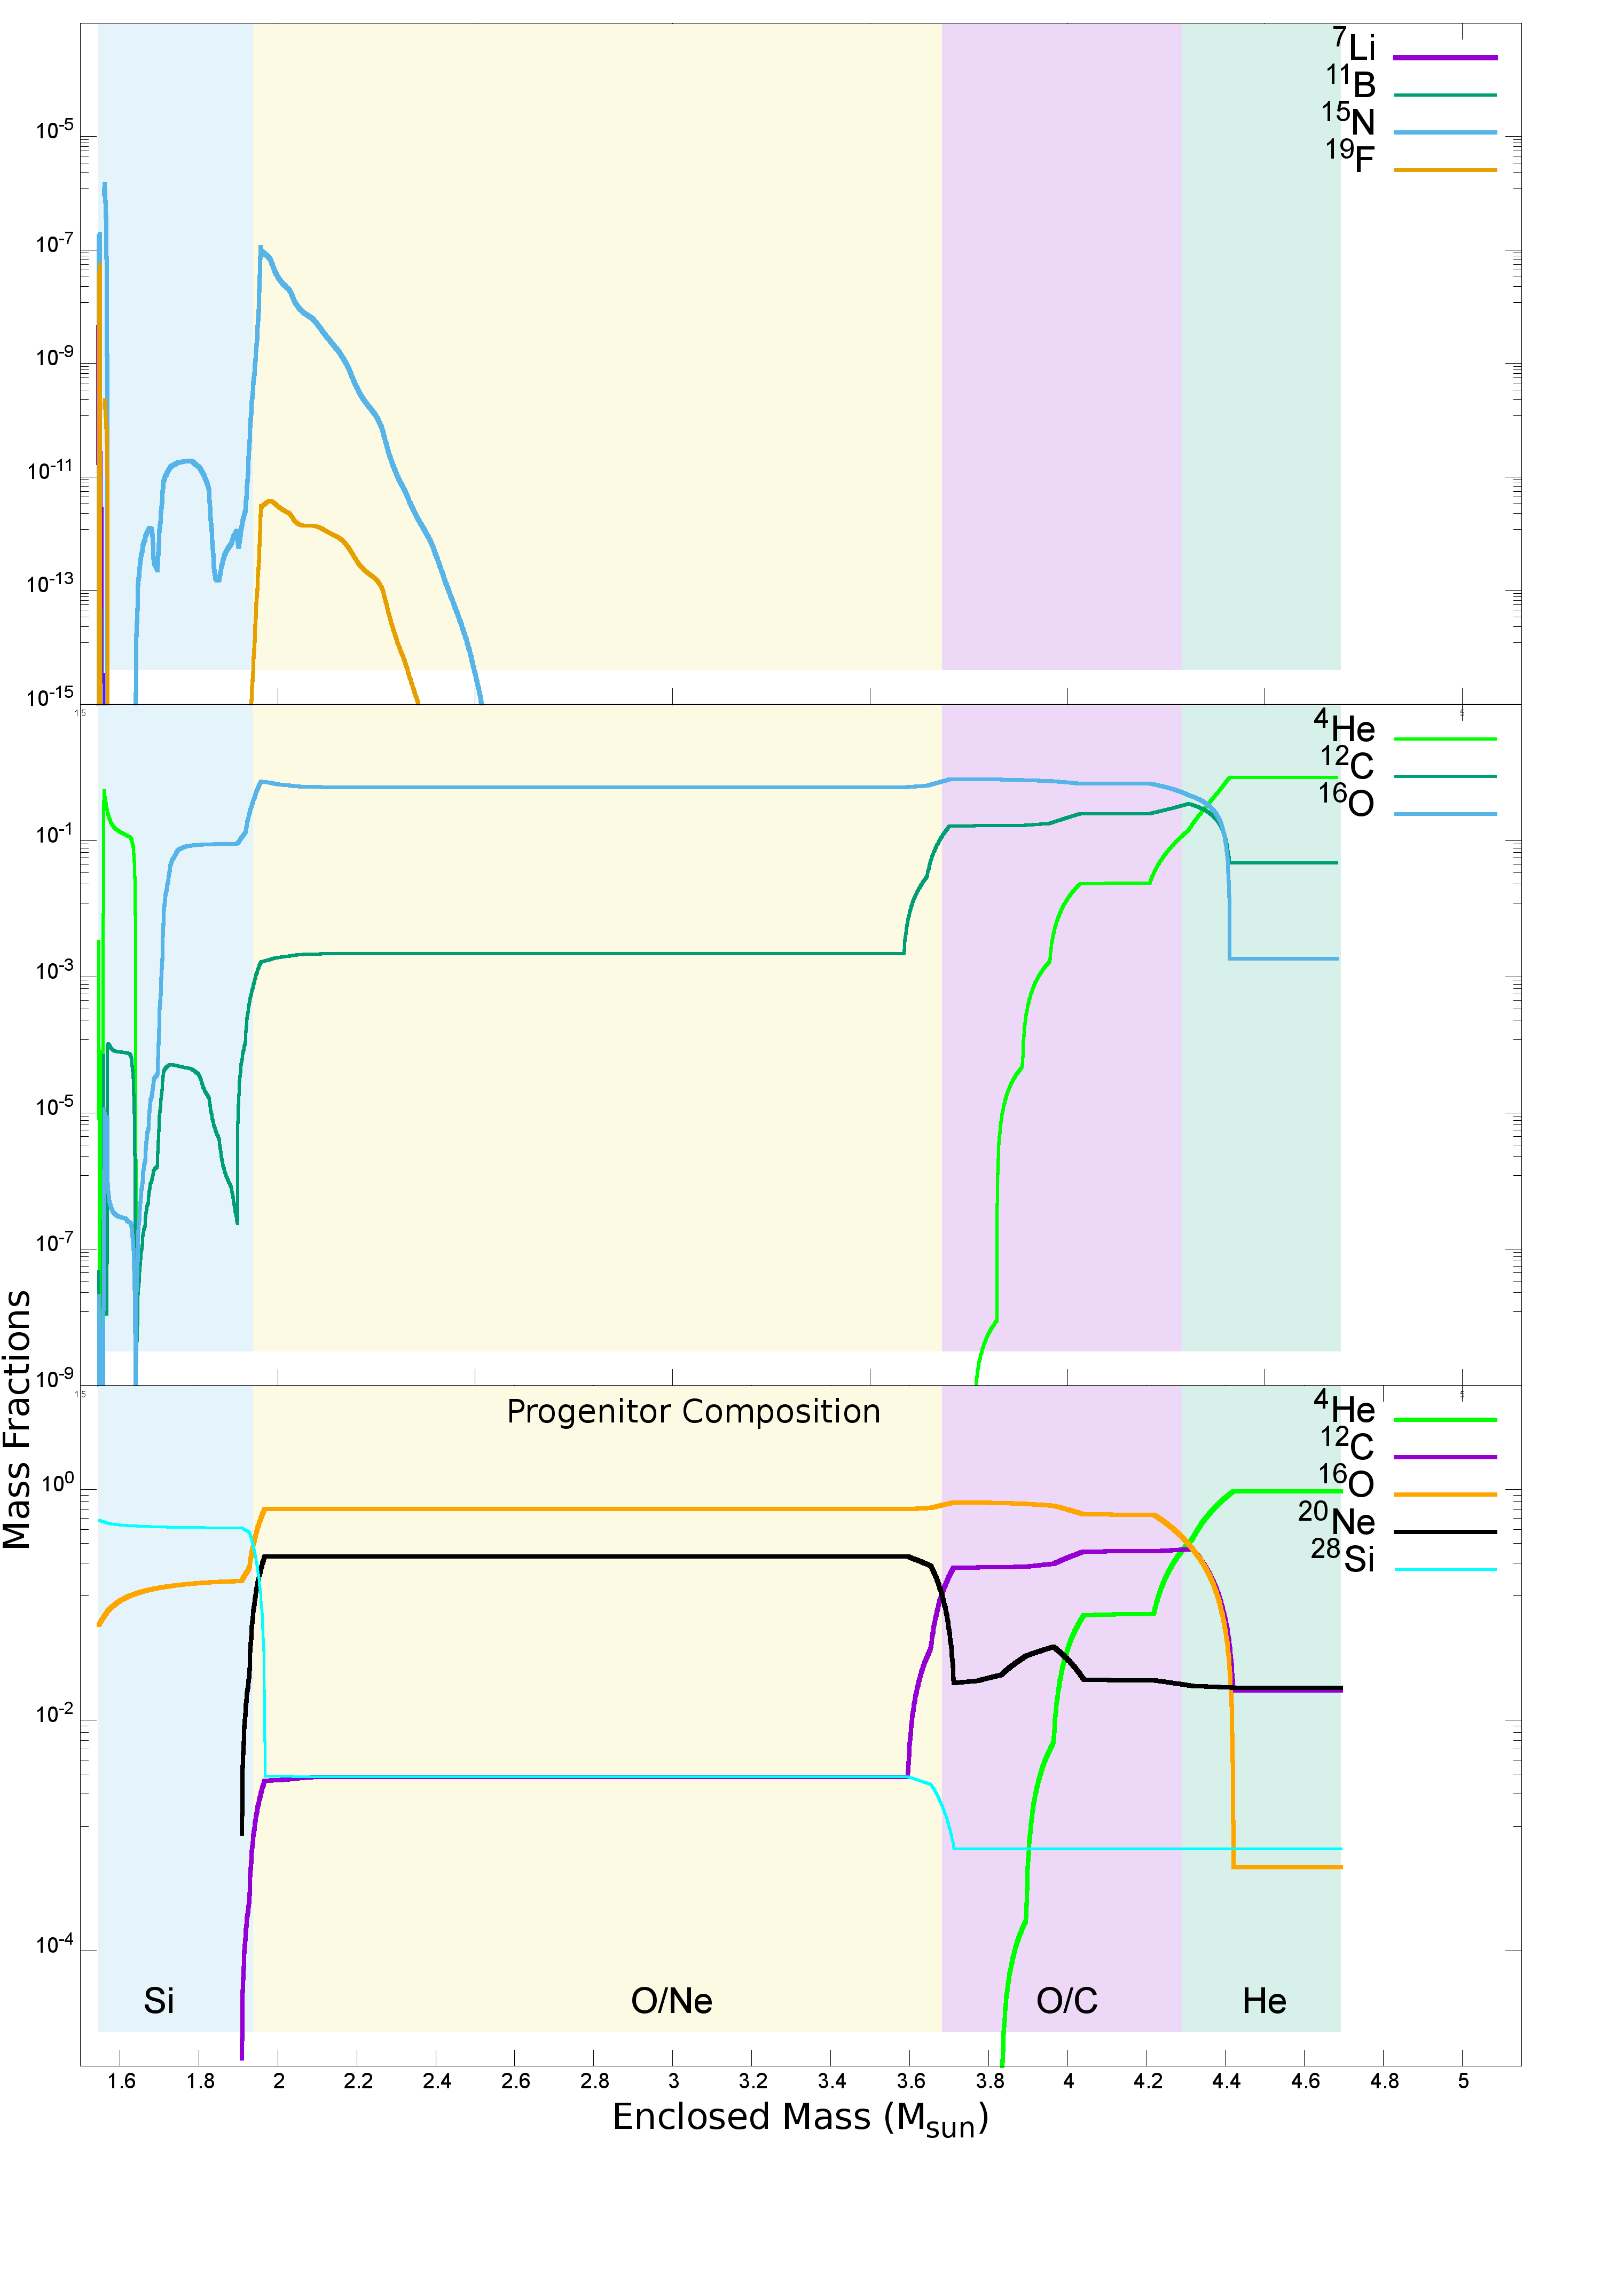
\includegraphics[width=\textwidth]{figures/abundadecay_noNu_he4li7b11c12n15o16f19_hor}
		\caption[Nötrino Sentezlenmesi İhmal Edildiğinde]{Nötrino sentezlenmesi ihmal edildiğinde}
	\end{subfigure}
%%%%%%%%%%%%%%
	\begin{subfigure}{.49\textwidth}
		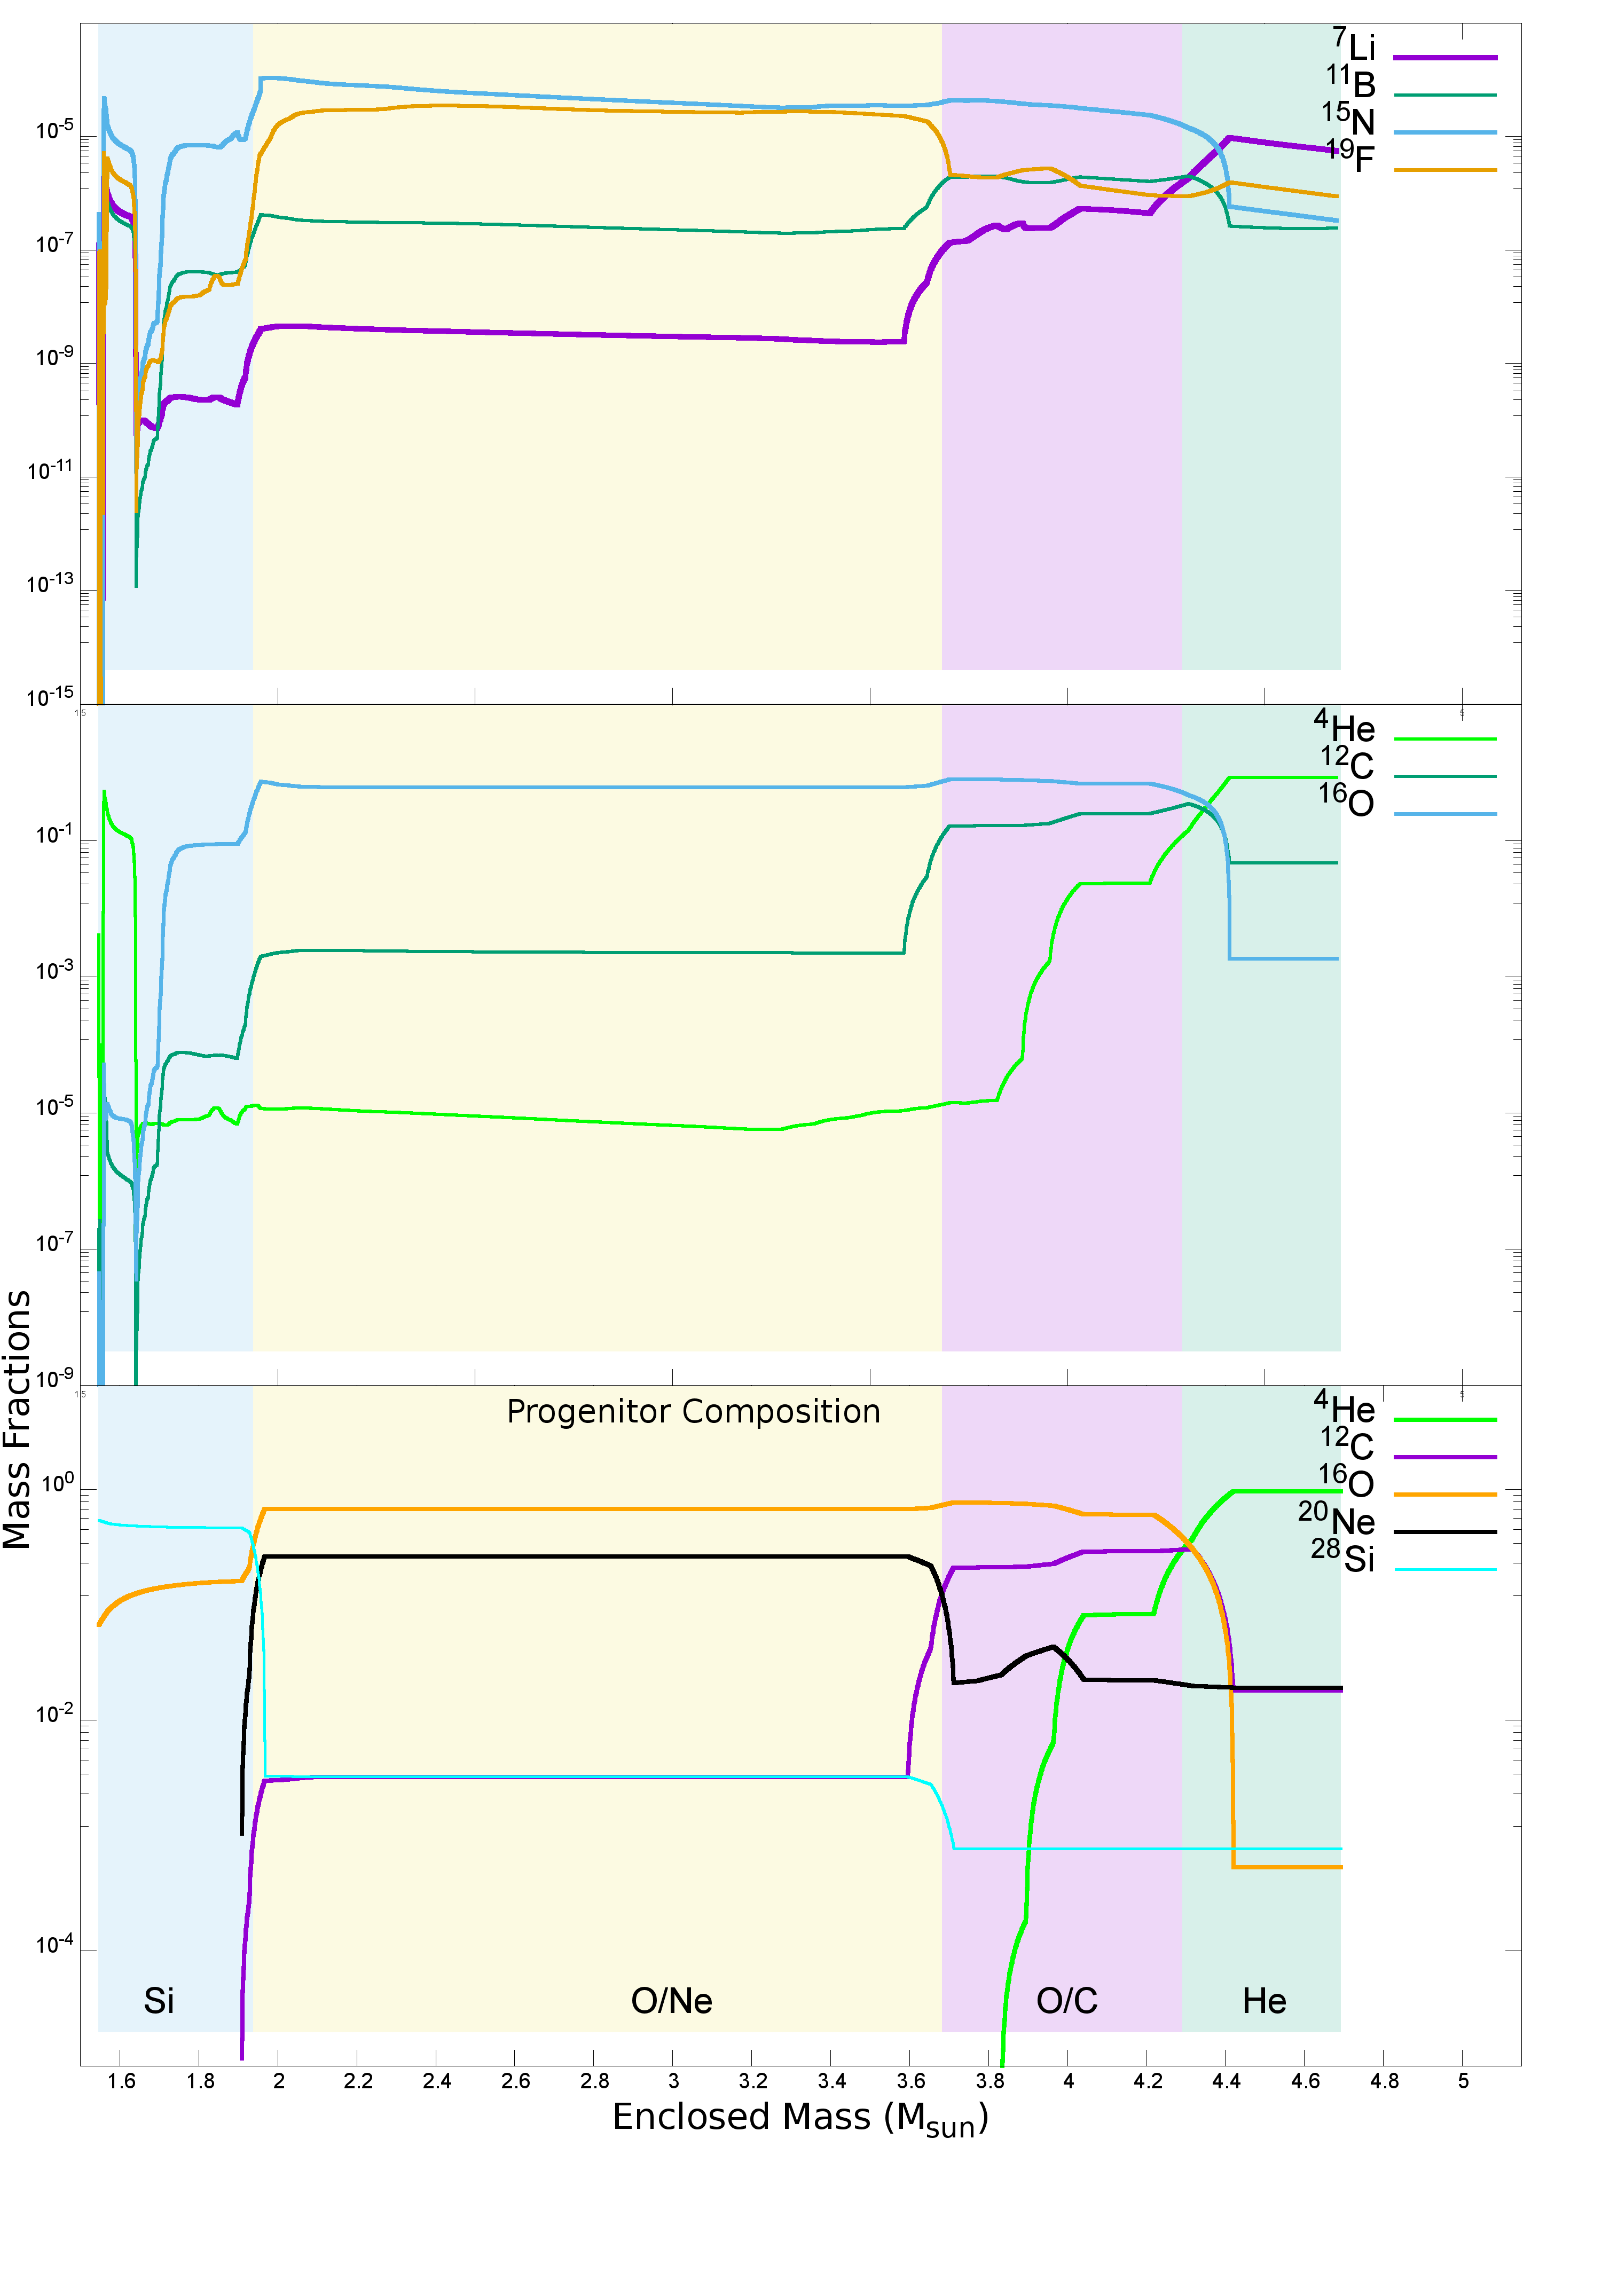
\includegraphics[width=\textwidth]{figures/abundadecay_he4li7b11c12n15o16f19_hor}
		\caption[Nötrino Sentezlenmesi Dahil Edildiğinde]{Nötrino sentezlenmesi dahil edildiğinde.}
	\end{subfigure}
%%%%%%%%%%%%%%
	\caption[Nötrinolu Ve Nötrinosuz Nötrino-işlem Çekirdeklerinin Kütle Kesirleri]{Nötrinolu ve nötrinosuz nötrino-işlem çekirdeklerinin kütle kesirleri.}
    \label{fig:he4li7b11c12n15o16f19_abund_comp}
\end{figure}

$18.8$ M$ _{\odot} $ kütleli PUSHing simülasyonu kullanılarak elde edilen bazı $ \nu $-işlem çekirdeklerinin, $ ^{7} $Li, $ ^{11} $B, $ ^{15} $N ve $ ^{19} $F, kütle kesirleri \ref{fig:he4li7b11c12n15o16f19_abund_comp} numaralı şekillerde verilmiştir. Bu şekillerde, nötrinolu ve nötrinosuz çekirdek sentezi arasındaki fark, O/Ne, O/C ve He kabuklarında açıkça gözükmektedir. Nötrino etkileşimleri dikkate alınmaz ise, yıldız içerisinde $ ^{7} $Li ve $ ^{11} $B izotopu sentezlenemez. Bu çekirdeklere ek olarak $ ^{15} $N ve $ ^{19} $F üretimi de nötrino varlığından etkilenir. Nötrino işlemi, bu çekirdeklerin üretimine $ ^{16} $O($ \nu $,$ \nu $'$ p/n $)$ ^{15} $N ve $ ^{20} $Ne($ \nu $,$ \nu $'$ p/n $)$ ^{19} $F tepkimeleri ile katkıda bulunur.

Şekillerdeki tüm kütle fraksiyonları değerleri, bozunmaların ardından elde edildiğini söylemek önemlidir. Bu, çekirdek sentezleme simülasyonun bitip $200$ saniye sonrasına kadar bozunma hesaplamalarının dahil edildiği anlamına gelir. Son olarak \ref{fig:he4li7b11c12n15o16f19_abund_comp} numaralı şekilde, nötrinoların O/Ne katmanında önemli miktarda $ ^{4} $He yani $ \alpha $ parçacıkları ürettiği görülür. Süpernova evrim simülasyonu $5$ saniye sürdüğü ve o anda şok dalgası O/Ne tabakasının sonuna ulaştığı için bu bölgedeki bolluklar nötrino işlem veya diğer tip işlem (n,p,$\nu$ p gibi) etkileşimlerle kolayca açıklanamaz. Şok dalgasının enerjisi ile bu noktadaki çekirdekler de parçalanır. Yani parçalanma (spallation) reaksiyonları çekirdek bolluğu ve çekirdek sentezleme hesaplarında önemli yer tutar. Bu çalışmada parçalanma etkisi dikkate alınmıştır.

Yük sayıları (charge number) göre tüm çekirdeklerin toplam ürünleri (yield) \ref{fig:abundadecay_Z_TotalYields_nu_nuNo} numaralı şekilde verilmiştir. Nötrino-çekirdek etkileşimleri çoğunlukla Li, Be, B ve F elementlerinin ve bunların izotoplarının üretimini önemli ölçüde etkiler. Tüm ürünler, kararsız $ ^{7} $Be ve $ ^{11} $C çekirdeklerinin bozunumundan önce hesaplanmıştır. \ref{fig:abundadecay_Z_TotalYields_nu_nuNo} numaralı şekilde, $ Z=4 $ ve $ Z=9 $ civarındaki ani artış, nötrino sürecinin kırılgan hafif elementlerin Güneş sistemindeki bolluğunu açıklamada umut vericidir. Ayrıca nötrino etkileşimleri yoluyla Be çekirdeğinin üretilmesi, Li ve B çekirdeklerinin toplam verimini değiştirir. Bunun iki nedeni vardır. Bunlardan en önemlisi, nötrinoların Be çekirdeğindeki proton/nötron sayısını değiştirmesi ve bunun sonucundaki beta bozunumlarıdır. Bir diğeri ise nötrinolar, yüksüz akım etkileşimleri yoluyla enerjilerini yıldız ortamına aktarmalarıdır. Bu aktarım elementlerin reaksiyon hızını da arttırır. Son olarak $ Z=50 $'nin ötesindeki küçük değişiklikler önemli değildir çünkü ata yıldızın bileşeninde ağır elementleri üretebilecek olan ağır izotoplar bulunmamaktadır.

\begin{figure}[hbt!]
    \centering
    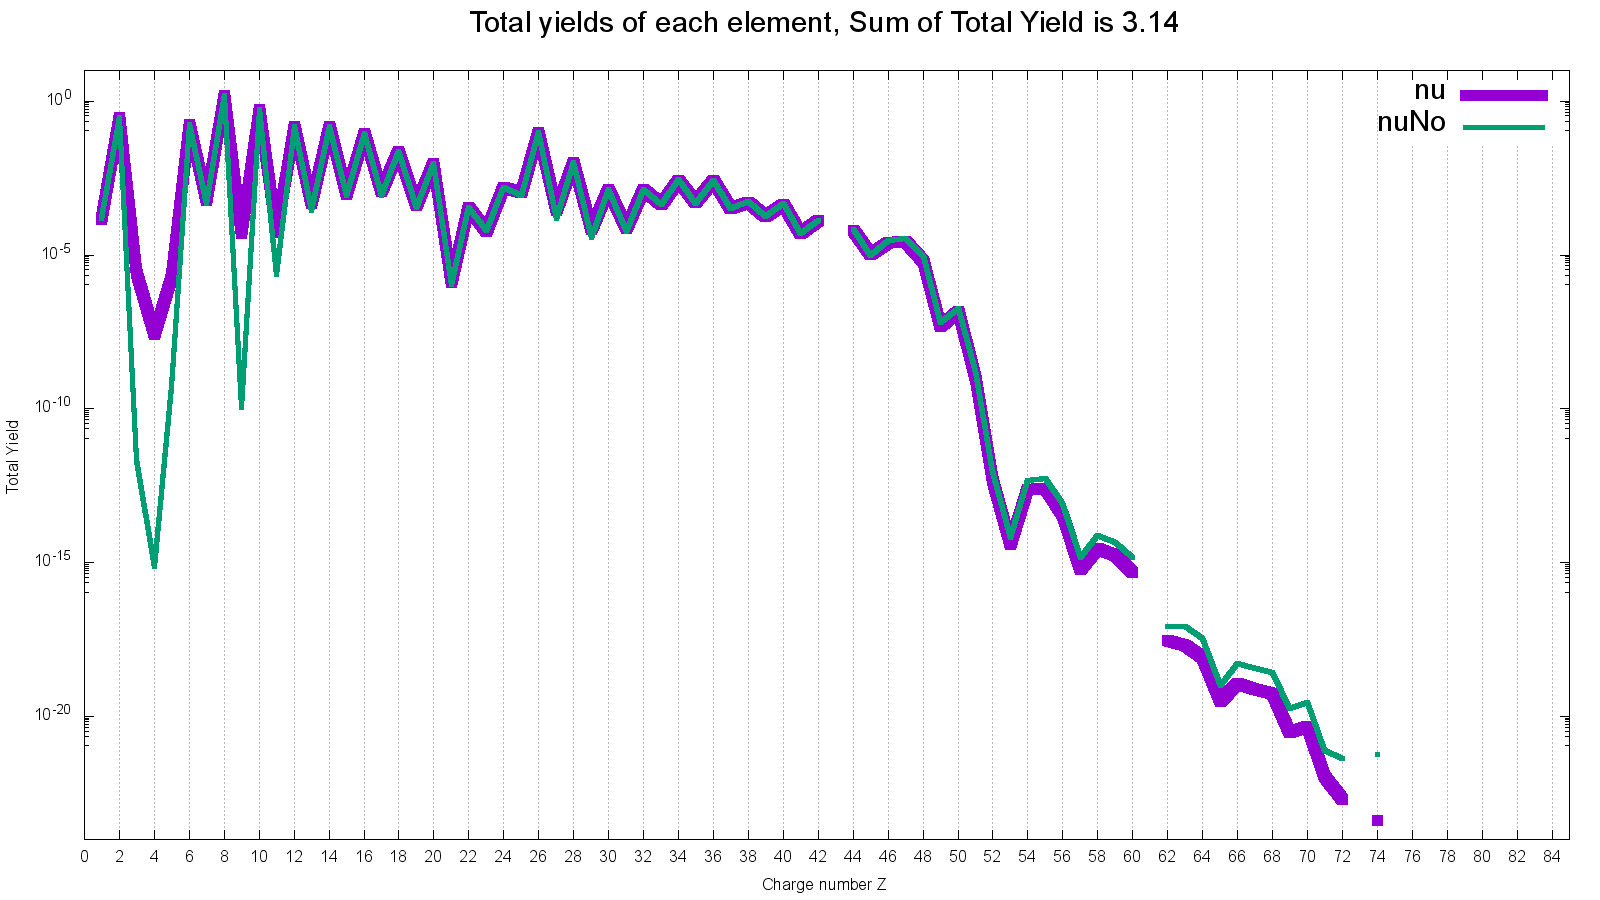
\includegraphics[width=1\textwidth]{figures/abundadecay_Z_TotalYields_nu_nuNo}
    \caption[Toplam Ürünün Yük Sayısı $ Z $'ye Göre Değişimi.]{Toplam ürünün yük sayısı $ Z $'ye göre değişimi. \emph{Nu} ile adlandırılan mor çizgiler nötrino etkileşimleri gözetildiğinde açığa çıkan toplam ürünleri, \emph{nuNo}" ise nötrino etkileşimlerinin ihmal edildiği durumda açığa çıkan toplam ürünleri gösterir.}
    \label{fig:abundadecay_Z_TotalYields_nu_nuNo}
\end{figure}